%
% File acl07.tex
%

\documentclass[11pt]{article}
\usepackage{acl08}

% hyperref clobbers acl08's citations style, so we fool it into not trying to much with cites.  (too bad it's one of the cooler features)
\makeatletter
\def\NAT@parse{\typeout{This is a fake Natbib command to fool Hyperref.}}
\makeatother
\usepackage{hyperref}
\hypersetup{colorlinks=false}
\newcommand{\hurl}[1]{\href{#1}{\scriptsize{\url{#1}}}}

\usepackage{times}
\usepackage{latexsym}
\usepackage{amsmath}
\usepackage{eucal}
\usepackage{eufrak}
\usepackage{mathrsfs}
\usepackage[dvips]{graphicx}
\usepackage[dvips]{epsfig}


\parskip=3pt
\abovedisplayskip 3.0pt plus2pt minus2pt%
\belowdisplayskip \abovedisplayskip
\renewcommand{\baselinestretch}{0.985}
\newlength{\sectionReduceTop}
\newlength{\sectionReduceBot}
\newlength{\abstractReduceTop}
\newlength{\abstractReduceBot}
\newlength{\captionReduceTop}
\newlength{\captionReduceBot}
\newlength{\nameReduceTop}
\newlength{\tableReduceTop}
\newlength{\tableReduceBot}
\setlength{\sectionReduceTop}{-0.2in}
\setlength{\sectionReduceBot}{-0.2in}
%\setlength\topmargin{0.8in}   % for box on top for blog post
\setlength{\tableReduceTop}{-0.00in}
\setlength{\tableReduceBot}{-0.10in}

\setlength{\captionReduceTop}{-0.15in}
\setlength{\captionReduceBot}{-0.25in}

\setlength{\nameReduceTop}{-0.05in}

\setlength{\abstractReduceTop}{-0.6in}
\setlength{\abstractReduceBot}{-0.15in}

\setlength\titlebox{7cm}    % Expanding the titlebox
%\setlength\titlebox{6.0cm}    % Expanding the titlebox

\title{Cheap and Fast  ---  But is it Good?\\Evaluating Non-Expert Annotations for Natural Language Tasks }

%
\author{Rion Snow$^\dagger$ \hspace{.3cm} Brendan O'Connor$^\ddagger$ \hspace{.3cm} Daniel Jurafsky$^\mathchar "278$ \hspace{.3cm} Andrew Y. Ng$^\dagger$ \\
\AND  \vspace{-0.35in} \\ $^\dagger$Computer Science Dept.\\
Stanford University \\
Stanford, CA 94305 \\
\footnotesize{\tt \{rion,ang\}@cs.stanford.edu}\\
%\scriptsize{\tt \{rion,ang\}@cs.stanford.edu}\\
\And   \vspace{-0.35in}\\
$^\ddagger$Dolores Labs, Inc.\\
832 Capp St. \\
San Francisco, CA 94110 \\
\footnotesize{\tt brendano@doloreslabs.com} \\
\And   \vspace{-0.35in} \\
$^\mathchar "278$Linguistics Dept. \\
Stanford University\\
Stanford, CA 94305 \\
\footnotesize{\tt jurafsky@stanford.edu} }

%\author{Rion Snow\\
%Computer Science Department \\
%\small{Computer Science Dept.}\\
%\affiliation{
% \begin{tabular}{cl}
% \dag & Stanford University \\
% \end{tabular}
%}

%\small{Stanford University} \\
%\small{Stanford, CA 94305} \\
%\And Brendan O'Connor\\
%\small{Dolores Labs, Inc.}\\
%%\small{832 Capp St.}\\
%\small{San Francisco, CA 94110} \\
%\scriptsize{\tt brendano@doloreslabs.com} \\
%\footnotesize{\tt www.anyall.org} \\
%\And Daniel Jurafsky       Andrew Y. Ng\\
%Linguistics Department\\
%Linguistics Dept.\\
%Stanford University\\
%Stanford, CA 94305 \\
%\scriptsize{\tt jurafsky@stanford.edu, ang@cs.stanford.edu} }
%\And Andrew Y. Ng\\
%Computer Science Department\\
%Computer Science Dept.\\
%Stanford University \\
%Stanford, CA 94305 USA \\
%Stanford, CA 94305 \\
%\scriptsize{\tt ang@cs.stanford.edu} }
%  Affiliation / Address line 1\\
%  Affiliation / Address line 2\\
%  Affiliation / Address line 3\\
%  {\tt email@domain}  \And
%  Sushant Prakash\\
%  Affiliation / Address line 1\\
%  Affiliation / Address line 2\
%  Affiliation / Address line 3\\
%  {\tt email@domain}}

 
\begin{document}
\maketitle

\vspace*{\abstractReduceTop}
\begin{abstract}
\small{Human linguistic annotation is crucial for many natural
language processing tasks but can be expensive and time-consuming.
We explore the use of Amazon's Mechanical Turk system, a significantly cheaper and faster method for collecting annotations from a broad base of paid non-expert contributors over the Web.  We investigate five tasks: affect recognition, word similarity, recognizing textual entailment, 
event temporal ordering, and word sense disambiguation.
For all five, we show high agreement between Mechanical Turk non-expert annotations
and existing gold standard labels provided by expert labelers.  
For the task of affect recognition, we also show that using non-expert
labels for training machine learning algorithms can be as effective
as using gold standard annotations from experts.  We propose a technique for bias correction that significantly improves annotation quality on two tasks.  We conclude that 
many large labeling tasks can be effectively designed and carried
out in this method at a fraction of the usual expense.}

%\small{ Large scale annotation projects have been crucial in influencing the direction of research in the statistical natural language processing community.  Such projects are often extremely expensive and have led many researchers to suggest the possibility of collecting annotations from a broad base of non-expert volunteer contributors over the Web. We explore the use of Amazon's Mechanical Turk system to study whether volunteers on the web can provide reliable annotations on a variety of natural language annotation tasks with high interannotator agreement compared to existing gold standard labels provided by expert labelers. The tasks include recognizing textual entailment, affect recognition, word similarity, temporal event annotation, and word sense disambiguation. We demonstrate that for a wide range of different natural language annotation tasks, averaging over annotations from labelers on Mechanical Turk can yield high quality annotations. We further provide an analysis of relative payment rates and strategies for minimizing the required number of annotators necessary for high quality annotations.  Finally we demonstrate that using Turker labels for training machine learning algorthms can be as effective as using gold standard annotations from experts.  We conclude that many large labeling tasks can be effectively designed and carried out in this method at a fraction of the usual monetary and temporal costs. }

%Many tasks in statistical natural language processing rely on the availability of manually annotated gold standard data.  
% The advent of widespread connectivity has made the power of distributed human computation easily available to anyone with a computer

\end{abstract}

\section{Introduction}

Large scale annotation projects such as TreeBank \cite{TreeBank}, PropBank \cite{PropBank}, TimeBank \cite{TimeBank}, FrameNet \cite{FrameNet}, SemCor
\cite{SemCor}, and others play an
important role in natural language processing research,
encouraging the development of novel ideas, tasks, and algorithms.
The construction of these datasets, however, is extremely expensive in both annotator-hours and financial cost.  Since the performance of many natural language processing tasks is limited by the amount
and quality of data available to them \cite{Banko:01}, one promising alternative for some tasks is the collection of non-expert annotations.

In this work we explore the use of Amazon Mechanical Turk\footnote{
%\texttt{\scriptsize{http://mturk.com.}}} 
\hurl{http://mturk.com}} (AMT) to determine whether non-expert labelers can provide reliable natural language annotations.
%Our goals are to produce high quality labels for a number of NLP tasks,
%to investigate which tasks are appropriate for this kind of annotation,
%and to develop the methodological framework for achieving high-accuracy labels.
We chose five natural language understanding tasks that we felt would be sufficiently natural and learnable for non-experts, and for which we had gold standard labels from expert labelers, as well as (in some cases) expert labeler agreement information.
The tasks are: affect recognition, word similarity, recognizing
textual entailment, event temporal ordering, and word sense
disambiguation.   For each task, we used AMT to annotate data and
measured the quality of the annotations by comparing them with the
gold standard (expert) labels on the same data. Further, we compare machine learning classifiers
trained on expert annotations vs. non-expert annotations.

In the next sections of the paper
we introduce the five tasks and the evaluation metrics, and offer
methodological insights, including a technique for bias correction
that improves annotation quality.\footnote{
Please see \hurl{http://blog.doloreslabs.com/?p=109} for a condensed version of this paper, follow-ups, and ongoing public discussion.  We encourage comments to be directed here in addition to email when appropriate.  Dolores Labs Blog, ``AMT is fast, cheap, and good for machine learning data,'' Brendan O'Connor, Sept.~9,~2008.  More related work at \hurl{http://blog.doloreslabs.com/topics/wisdom/}.}

%
%Large scale annotation projects such as TreeBank \cite{TreeBank}, FrameNet \cite{FrameNet}, ProbBank \cite{PropBank}, SemCor \cite{SemCor} and many others have played an important role in influencing the direction of research in the statistical natural language processing community.  The construction of large manually-annotated gold-standard datasets has allowed researchers to explore and evaluate a variety of novel ideas and algorithms for solving different tasks.  However, the construction of these datasets is often extremely expensive, in terms of both annotator-hours and monetary expense.  The prospect of collecting annotations from non-expert volunteer contributors has been lauded as a promising alternative to this laborious process for certain tasks where the annotator requires only language fluency; however, the problem of drawing sufficient non-expert annotators to one's task is non-trivial.  

%In this work we explore the use of the Amazon Mechanical Turk system\footnote{Amazon Mechanical Turk may be found online at http://mturk.com.} (AMT) to study whether non-expert volunteers on the web can provide reliable annotations on a variety of natural language annotation tasks.  We measure the quality of the annotations with respect to expert interannotator agreement compared to existing gold standard labels provided by expert labelers. The tasks we explore include affect recognition, word similarity, recognizing textual entailment, temporal event annotation, and word sense disambiguation. We demonstrate that for a wide range of different natural language annotation tasks, averaging over annotations from labelers on AMT can yield high quality annotations. We further provide an analysis of relative payment rates and strategies for minimizing the required number of annotators necessary for high quality annotations.  Finally we demonstrate that using Turker labels for training machine learning algorthms can be as effective as using gold standard annotations from experts.  We conclude that many large labeling tasks can be effectively designed and carried out in this method at a fraction of the typical monetary and temporal cost.

%[[ Many tasks in natural language processing have a data bottleneck. ]]

%[[ The performance of statistical methods in natural language processing are frequently limited by the amount and quality of data available to them. ]]

%[[ Labeling data is hard and expensive.  Volunteers from the internet are plentiful.  Many tasks are simple, but not necessarily fun -- paying a small amount of money is sufficient for attracting annotators to simple but not-very-fun tasks. ]]

%[[ Optional: Rather than only being a method for collecting final annotations, AMT may also be used as a cost-effective means to perform user studies for annotation tasks across a wider population;  when developing guidelines Some things you can do with Mechanical Turk:  while considering the actual.  \cite{CorbettBlog:07} writes on the experience of developing a set of guidelines for annotating chemical named entities in scientific text \cite{Corbett:07}, writes that:  ``Having some framework where I could make variations in the annotation guidelines, re-annotate a corpus and see how it affects a task which can be evaluated against some ‘wild’ data would be very helpful in evaluating the guidelines."  Services like Mechanical Turk make tasks such as this not only possible, but also cost-effective.]]

%, TREC \cite{TREC} 

\section{Related Work}

The idea of collecting annotations from volunteer contributors has been used for a variety
of tasks. Luis von Ahn pioneered the collection of data via online
annotation tasks in the form of games, including the ESPGame for
labeling images \cite{espgame} and Verbosity for annotating word
relations \cite{verbosity}.  The Open Mind Initiative \cite{OpenMind}
has taken a similar approach, attempting to make such tasks as
annotating word sense \cite{WordExpert} and common-sense word
relations \cite{OpenMindCommonSense} sufficiently ``easy and fun''
to entice users into freely labeling data.

There have been an increasing number of experiments using Mechanical
Turk for annotation.  In \cite{Su:07} workers provided annotations for the tasks of
hotel name entity resolution and attribute extraction of age, product brand, and
product model, and were found to have high accuracy compared to gold-standard labels.  
\newcite{Kittur:08} compared AMT evaluations of Wikipedia article quality against experts, finding validation tests were important to ensure good results.
\newcite{Zaenen:08} studied the agreement of annotators
on the problem of recognizing textual entailment (a similar task
and dataset is explained in more detail in Section 4).

At least several studies have already used AMT without external gold standard comparisons.
In \cite{NakovLREC:08} workers generated paraphrases of 250 noun-noun compounds which were then used
as the gold standard dataset for evaluating an automatic method of noun compound paraphrasing.
% bto; note sure whether to mention or replace with NakovACL:08
\newcite{Kaisser:08a} use AMT to help build a dataset for question answering, 
%. Following on
%to corpora constructed for the TREC QA Evaluation \cite{Voorhees:06},
%where answers to factoid questions are annotated at the document
%level, \cite{Kaisser:08a} used AMT to annotate the answers to 8107
annotating the answers to 8107
questions with the \textit{sentence}
containing the answer.  
\newcite{Kaisser:08b} examines the task of
customizing the summary length of QA output;
non-experts from AMT chose a summary length that suited their information needs for varying
query types.  
\newcite{Dakka:08} evaluate a document facet generation system against AMT-supplied facets, and also use workers for user studies of the system.  \newcite{Sorokin:08} collect data for machine vision tasks and report speed and costs similar to our findings; their summaries of worker behavior also corroborate with what we have found.

In general, volunteer-supplied or AMT-supplied data is more plentiful but noisier than expert data.  It is powerful because independent annotations can be aggregated to achieve high reliability.  \newcite{Sheng:08} explore several methods for using many noisy labels to create labeled data, how to choose which examples should get more labels, and how to include labels' uncertainty information when training classifiers.  Since we focus on empirically validating AMT as a data source, we tend to stick to simple aggregation methods.

\section{ Task Design }

In this section we describe Amazon Mechanical Turk and the general design of our experiments.

\subsection{ Amazon Mechanical Turk }

We employ the Amazon Mechanical Turk system in order to elicit annotations from non-expert labelers.  %BTO i figure we should say it isn't a "volunteer" system really so 1 sentence:
AMT is an online labor market where workers are paid small amounts of money to complete small tasks.  The design of the system is as follows: one is required to have an Amazon account to either submit tasks for annotations or to annotate submitted tasks.  These Amazon accounts are anonymous, but are referenced by a unique Amazon ID.  A \textit{Requester} can create a \textit{group} of \textit{Human Intelligence Tasks} (or \textit{HIT}s), each of which is a form composed of an arbitrary number of questions.  The user requesting annotations for the group of HITs can specify the number of unique annotations per HIT they are willing to pay for, as well as the reward payment for each individual HIT.  While this does not guarantee that unique people will annotate the task (since a single person could conceivably annotate tasks using multiple accounts, in violation of the user agreement), this does guarantee that annotations will be collected from unique accounts.  AMT also allows a requester to restrict which workers are allowed to annotate a task by requiring that all workers have a particular set of qualifications, such as sufficient accuracy on a small test set or a minimum percentage of previously accepted submissions.  Annotators (variously referred to as \textit{Workers} or \textit{Turkers}) may then annotate the tasks of their choosing. Finally, after each HIT has been annotated, the Requester has the option of approving the work and optionally giving a bonus to individual workers. There is a two-way communication channel between the task designer and the workers mediated by Amazon, and Amazon handles all financial transactions.
 
%[[Describe Mechanical Turk -- history, how it works, how users are paid, etc. ]]
\vspace*{-0.05in}
\subsection{ Task Design }

In general we follow a few simple design principles:  we attempt to keep our task descriptions as succinct as possible, and we attempt to give demonstrative examples for each class wherever possible.  We have published the full experimental design and the data we have collected for each task online\footnote{All tasks and collected data are available at \hurl{http://ai.stanford.edu/\~rion/annotations/}.}.  We have restricted our study to tasks where we require only a multiple-choice response or numeric input within a fixed range. For every task we collect ten independent annotations for each unique item; this redundancy allows us to perform an in-depth study of how data quality improves with the number of independent annotations.

%[[other citations:   \cite{Chklovski:05} has specifically studied the annotation process for collecting labels on a meronym task volunteers over the web, and suggests a three-stage approach consisting of evaluation, retuning, and publication...]]

%[[possible other citations:  \cite{Sheng:08}.  BTO: can't find a place for it to fit, it's about a slightly different topic; given noisy labels, how useful are they and what's a good data collection/usage strategy?  i tried further down in the bias correction section,  but left it commented out, didnt fit there either
 \vspace*{-0.05in}
\section{ Annotation Tasks }

We analyze the quality of non-expert annotations on five tasks:
affect recognition, word similarity, recognizing textual entailment,
temporal event recognition, and word sense disambiguation. In this
section we define each annotation task and the parameters of the
annotations we request using AMT.  Additionally we give an initial
analysis of the task results, and summarize the cost of the experiments.
\subsection{ Affective Text Analysis }

This experiment is based on the affective text annotation task proposed in \newcite{AffectiveText}, wherein each annotator is presented with a list of short headlines, and is asked to give numeric judgments in the interval [0,100] rating the headline for six emotions: anger, disgust, fear, joy, sadness, and surprise, and a single numeric rating in the interval [-100,100] to denote the overall positive or negative \textit{valence} of the emotional content of the headline, as in
this sample headline-annotation pair:
\begin{center} \textbf{Outcry at N Korea `nuclear test'} \end{center}
\begin{equation*}
\begin{array}{ll}
&\small(\textit{Anger, 30}),(\textit{Disgust,30}),(\textit{Fear,30}), (\textit{Joy,0}),\\
&\small(\textit{Sadness,20}),(\textit{Surprise,40}),(\textit{Valence,-50}).
\end{array}
\end{equation*}
For our experiment we select a 100-headline sample from the original SemEval test set, and collect 10 affect annotations for each of the seven label types, for a total of 7000 affect labels.

%This task is attractive both because it can be described to annotators with only a few lines of instruction, and because we have a set of 1000 headlines that were each annotated by six experts for all seven affect types, allowing a rich study of the relative quality of expert and non-expert annotation.

%Example annotation:
%Headline:  ``Outcry at N Korea 'nuclear test' ''
%Sample annotations:
%
%\begin{table}[h]
%\footnotesize
%    \begin{center}
%	\begin{tabular}{|c||c c c c|}
%	\hline
%	Headline &  ``Outcry at N Korea `nuclear test' '' & & &  \\
%	\end{tabular}
%        \begin{tabular}{|c|c|c|c|c|c|c|}
%        \hline
%Anger & Disgust & Fear & Joy & Sadness & Surprise & Valence \\
%	\hline
%30 & 30 & 30 & 0 & 20 & 40 & -50\\
%        \hline
%        \end{tabular}
%    \caption{Sample affect annotation for one headline}\label{exampleAFF}
%\end{center}
%\end{table}

%
%Anger:  30
%Disgust: 30
%Fear: 30
%Joy: 0
%Sadness: 20
%Surprise: 40
%Valence: -50

%\footnote{Our affective text annotation task design has been anonymously published at http://nlpannotations.googlepages.com/affect\_sample.html.}

%Stats:
%Total labels
%Cost / label
%Average time / label
%
%\begin{table}[h]
%\footnotesize
%    \begin{center}
%        \begin{tabular}{|c||c|c|c|c|c|}
%        \hline
%        & Total & Labels &Cost & Time & Labels & Labels \\
%        Task & Labels  & per hit & (USD) & (hrs) & per USD & per hr \\
%        \hline
%        Affect & 7000 & 2.0 & 5.93 & 3500 & 1180.4 \\
%        \hline
%        \end{tabular}
%    \caption{Annotation details for affect recognition}\label{detailsAFF}
%\end{center}
%\end{table}

%Since we have each of six experts' annotations for the affective text analysis we are able to do the most thorough analysis of non-expert agreement.  

We then performed two comparisons to evaluate the quality of the AMT annotations.
First, we  asked how well the non-experts agreed with the experts.
We did this by comparing the interannotator agreement (ITA) of
individual expert annotations to that of single non-expert and
averaged non-expert annotations.  In the original experiment ITA
is measured by calculating the Pearson correlation of one annotator's
labels with the average of the labels of the other five annotators. For each expert labeler, we computed this ITA score of the expert against the other five;
we then average these ITA scores across all expert annotators to compute the average expert ITA  (reported in Table \ref{affectITA1} as ``E vs. E''.   We then do the same for individual non-expert annotations, averaging Pearson correlation across all sets of the five expert labelers (``NE vs. E'').  We then calculate the ITA for each expert vs. the averaged labels from all other experts and non-experts (marked as ``E vs. All'') and for each non-expert vs. the pool of other non-experts and all experts (``NE vs. All'').  We compute these ITA scores for each emotion task separately, averaging the six emotion tasks as ``Avg. Emo'' and the average of all tasks as ``Avg. All''.

%[[Table :: for each emotion, average agreement of averaged Turk vs. 5 experts, compare to average agreement of expert vs. 5 experts. And graphs. ]]

%perhaps:  exp. vs. expert... exp vs. all, non-exp vs. non-expert... vs. all across the top?
%and emotions down the vertical? cooool.
\begin{table}[h]
\footnotesize
    \begin{center}
        \begin{tabular}{|c||c|c||c|c|}
        \hline
	 Emotion &      \scriptsize   E vs. E &    \scriptsize    E vs. All &     \scriptsize   NE vs. E &    \scriptsize    NE vs. All\\
        \hline \footnotesize
        Anger & 0.459 & 0.503 & 0.444 & 0.573 \\
        Disgust & 0.583 & 0.594 & 0.537 & 0.647 \\
        Fear & 0.711 & 0.683 & 0.418 & 0.498 \\
        Joy & 0.596 & 0.585 & 0.340 & 0.421 \\
        Sadness & 0.645 & 0.650 & 0.563 & 0.651 \\
        Surprise & 0.464 & 0.463 & 0.201 & 0.225 \\
        Valence & 0.759 & 0.767 & 0.530 &  0.554 \\
        \hline
        Avg. Emo & 0.576 & 0.603 & 0.417 & 0.503 \\
        Avg. All & 0.580 & 0.607 &  0.433 &  0.510 \\
        \hline
%        Fear & Joy & Sadness & Surprise & Valence \\
%        \hline
%        0.459 & 0.583 & 0.711 & 0.596 & 0.645 & 0.464 & 0.759 \\
%        \end{tabular}
  %     \hline
        
   %     Nonexpert Interannotator Agreement\\
   %     \hline
   %     \begin{tabular}{|c|c|c|c|c|c|c|}
   %     Non-expert &  & & & & & & \\
   %     \hline
        \end{tabular}
    \caption{Average expert and non-expert ITA on test-set}\label{affectITA1}
\end{center}
\end{table}
%\vspace*{\tableReduceBot}

The results in Table \ref{affectITA1} conform to the expectation that experts are better labelers: experts
agree with experts more than non-experts agree with experts, although the ITAs are in many cases quite close. But we also found that adding non-experts to the gold standard (``E vs. All'')
improves agreement, suggesting that non-expert annotations are good enough
to increase the overall quality of the gold labels.
Our first  comparison showed that individual experts were better than individual non-experts.
In our next comparison we ask how many averaged non-experts it would take to rival the performance of a single expert.
We did this by averaging the labels of each possible subset of $n$ non-expert annotations, for value of $n$ in $\{1, 2, \ldots, 10\}$.  We then treat this average as though it is the output of a single `meta-labeler', and compute the ITA with respect to each subset of five of the six expert annotators.  We then average the results of these studies across each subset size; the results of this experiment are given in Table \ref{affectITA2} and in Figure \ref{affITAfigure}.  In addition to the single meta-labeler, we ask:  what is the minimum number of non-expert annotations $k$ from which we can create a meta-labeler that has equal or better ITA than an expert annotator?  In Table \ref{affectITA2} we give the minimum $k$ for each emotion, and the averaged ITA for that meta-labeler consisting of $k$ non-experts (marked ``$k$-NE'').  In Figure \ref{affITAfigure} we plot the expert ITA correlation as the horizontal dashed line.

\begin{table}[h]
\footnotesize
    \begin{center}
        \begin{tabular}{|c||c|c|c|c|}
        \hline
        Emotion & 1-Expert & 10-NE & $k$ & $k$-NE \\
        \hline
        Anger & 0.459 &  0.675 & 2 & 0.536 \\
        Disgust & 0.583 & 0.746 & 2 & 0.627 \\
        Fear & 0.711 & 0.689 &-- & -- \\
        Joy & 0.596 & 0.632  & 7 & 0.600 \\
        Sadness & 0.645 & 0.776 & 2 & 0.656 \\
        Surprise & 0.464 & 0.496 & 9 & 0.481 \\
        Valence & 0.759 & 0.844 & 5 & 0.803\\
        \hline
        Avg. Emo. & 0.576 & 0.669 & 4 & 0.589 \\
        Avg. All & 0.603 & 0.694 & 4 & 0.613 \\  %BTO typo
        \hline
        \end{tabular}
    \caption{Average expert and averaged correlation over 10 non-experts on test-set.  $k$ is the minimum number of non-experts needed to beat an average expert.}\label{affectITA2}
\end{center}
\vspace*{-0.1in}
\end{table}
\vspace*{\tableReduceBot}
These results show that for all tasks except ``Fear'' we are able to achieve expert-level ITA with the held-out set of experts within 9 labelers, and frequently within only 2 labelers.  Pooling judgments across all 7 tasks we find that on average it requires only 4 non-expert annotations per example to achieve the equivalent ITA as a single expert annotator. Given that we paid US\$2.00 in order to collect the 7000 non-expert annotations, we may interpret our rate of 3500 non-expert labels per USD as at least 875 expert-equivalent labels per USD.

\begin{figure}[ht]
\centering
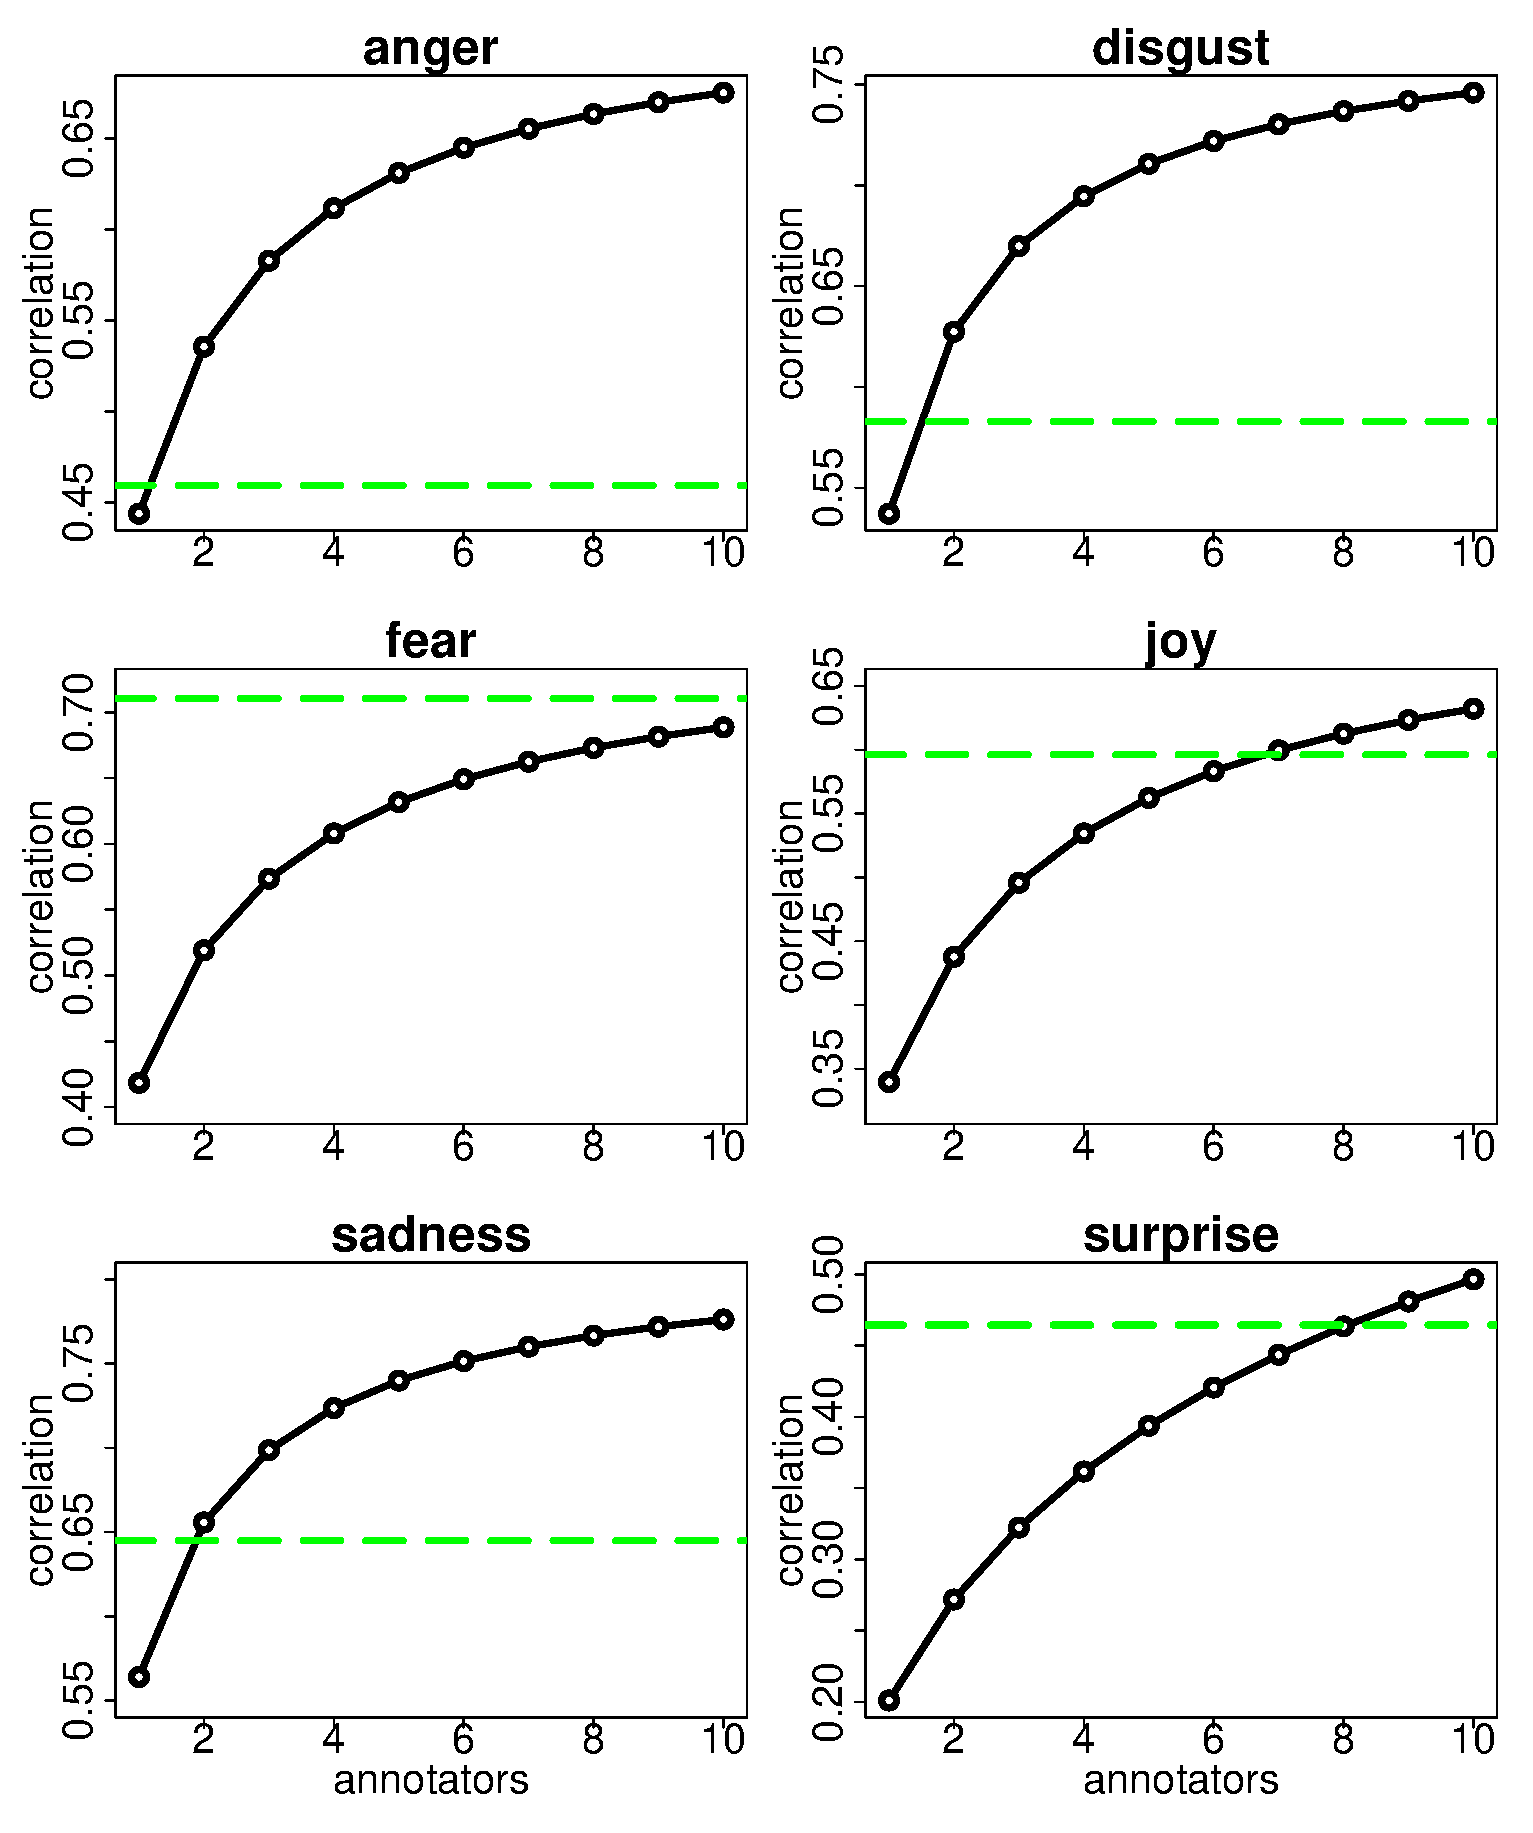
\includegraphics[width=8cm]{figures/all_emo.eps}
\caption{Non-expert correlation for affect recognition } \label{affITAfigure}
\end{figure}
\vspace*{-0.1in}
%Total annotations:  7000
%Total time: 5.93 hours
%Total cost:  \$2.00
%Avg anno / hour:  1180.4 anno /hour
%Avg anno / dollar: 3500 / 1 dollar
%Avg human-equiv labels / time:  
%Avg human-equiv labels / cost:  

\subsection{ Word Similarity }

This task replicates the word similarity task used in \cite{MC}, following a previous task initially proposed by \cite{RG}.  Specifically, we ask for numeric judgments of word similarity for 30 word pairs on a scale of [0,10], allowing fractional responses\footnote{\cite{MC} and others originally used a numerical score of [0,4].}.  These word pairs range from highly similar (e.g., \{\textit{boy, lad}\}), to unrelated (e.g., \{\textit{noon, string}\}).  Numerous expert and non-expert studies have shown that this task typically yields very high interannotator agreement as measured by Pearson correlation; \cite{MC} found a 0.97 correlation of the annotations of 38 subjects with the annotations given by 51 subjects in \cite{RG}, and a following study \cite{Resnik:99} with 10 subjects found a 0.958 correlation with \cite{MC}.

In our experiment we ask for 10 annotations each of the full 30 word pairs, at an offered price of \$0.02 for each set of 30 annotations (or, equivalently, at the rate of 1500 annotations per USD).  The most surprising aspect of this study was the speed with which it was completed; the task of 300 annotations was completed by 10 annotators in less than 11 minutes from the time of submission of our task to AMT, at the rate of 1724 annotations / hour.

As in the previous task we evaluate our non-expert annotations by averaging the numeric responses from each possible subset of $n$ annotators and computing the interannotator agreement with respect to the gold scores reported in \cite{MC}.  Our results are displayed in Figure \ref{wordsimITA}, with Resnik's 0.958 correlation plotted as the horizontal line; we find that at 10 annotators we achieve a correlation of 0.952, well within the range of other studies of expert and non-expert annotations.

%\begin{figure}[ht]
%\centering
%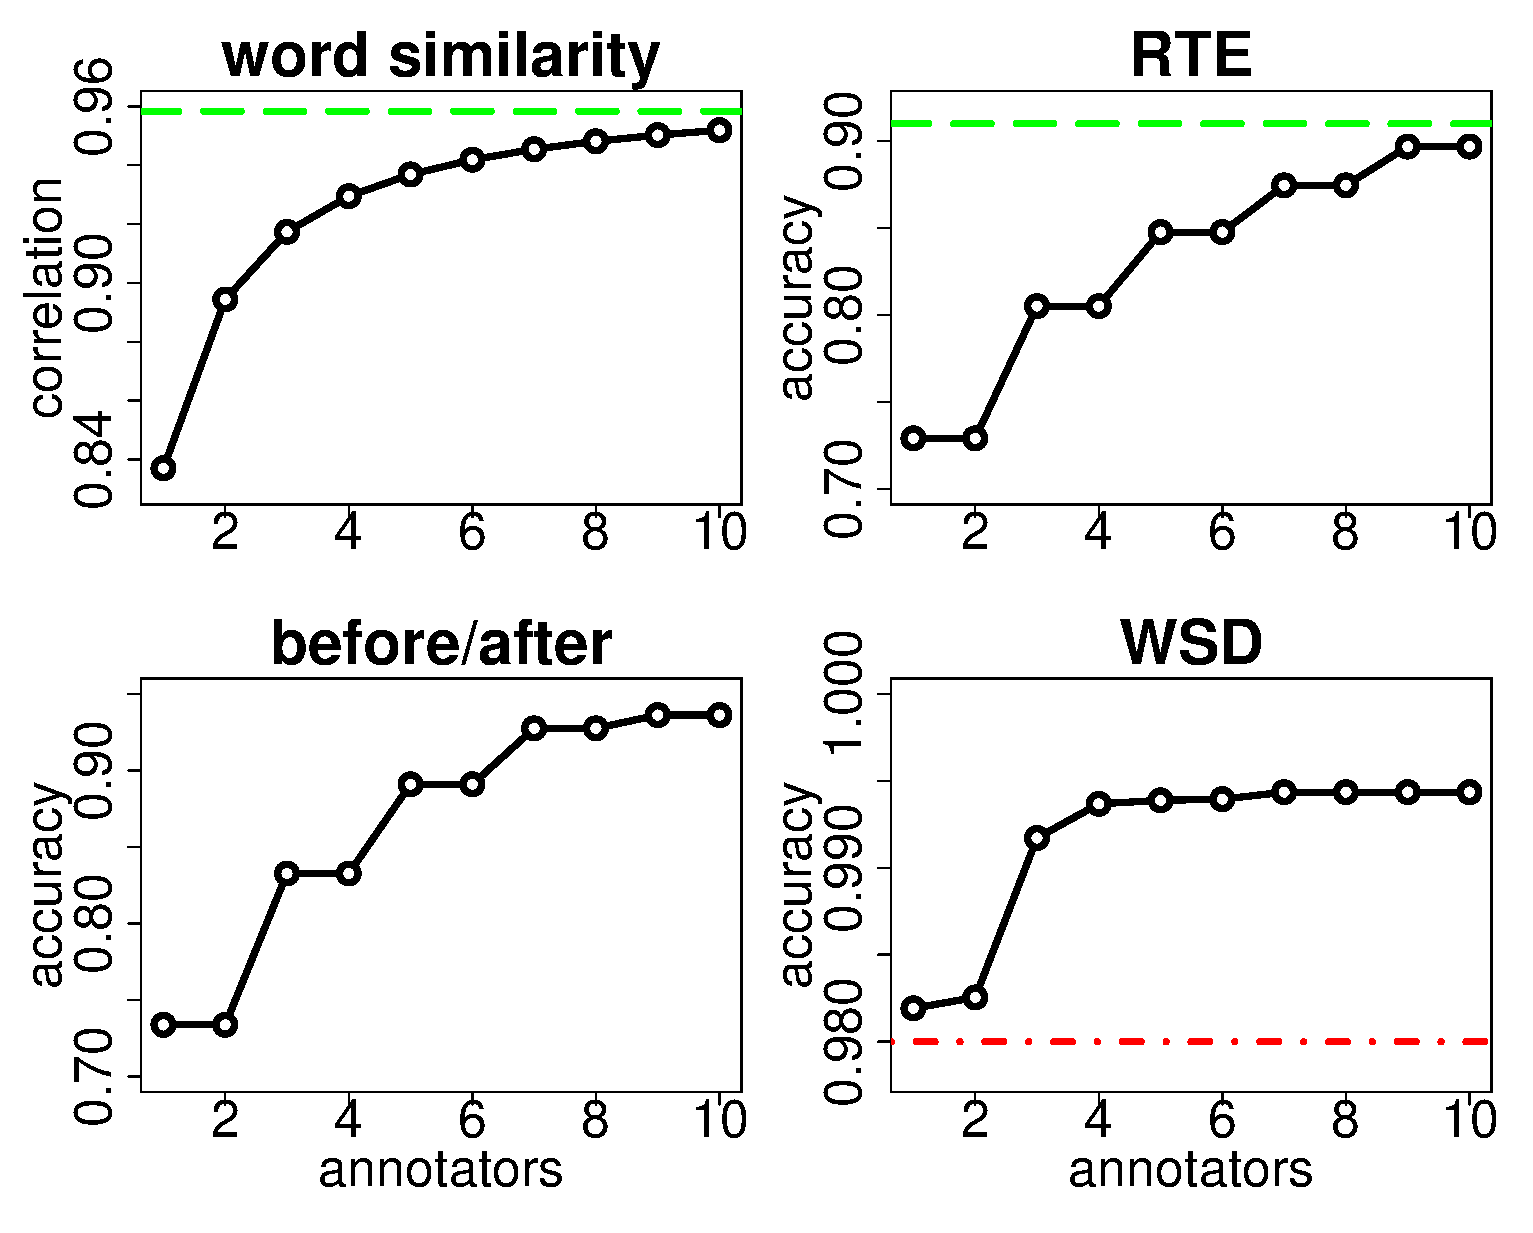
\includegraphics[width=8cm]{figures/all_rest.eps}%
%\caption{Inter-annotator correlation for word similarity, and agreement for RTE, event annotation, and %WSD tasks } \label{restITA}
%\end{figure}

\begin{figure}[ht]
\centering
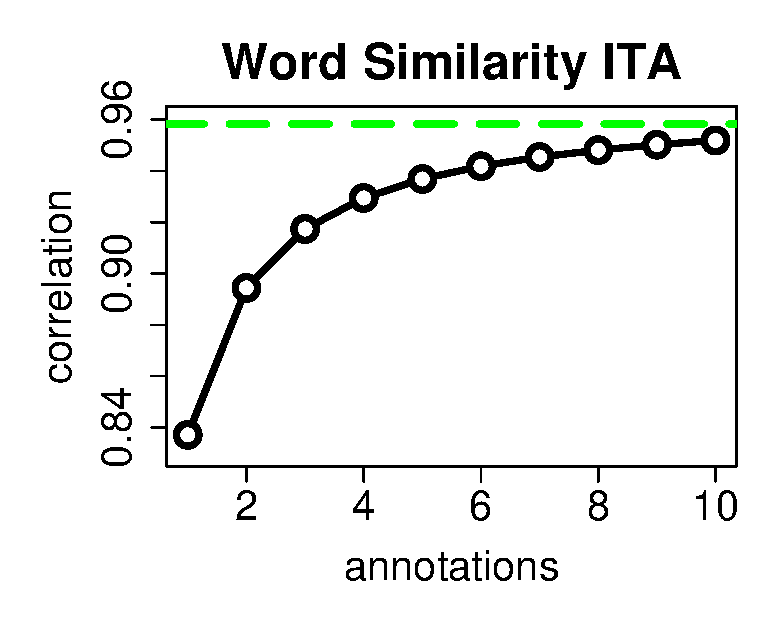
\includegraphics[width=7cm]{figures/wordsim.eps}
\caption{ITA for word similarity experiment } \label{wordsimITA}
\end{figure}

%We can also compare our results against the best current automatic systems for predicting human similarity rates; one such system is \cite{YP}, which 

\subsection{ Recognizing Textual Entailment }

This task replicates the recognizing textual entailment task originally proposed in the PASCAL Recognizing Textual Entailment task \cite{rte1}; here for each question the annotator is presented with two sentences and given a binary choice of whether the second \textit{hypothesis} sentence can be inferred from the first.  For example, the hypothesis sentence ``\textit{Oil prices drop}'' would constitute a \textit{ true entailment } from the text ``\textit{Crude Oil Prices Slump}'', but a \textit{false entailment} from ``\textit{The government announced last week that it plans to raise oil prices}''. 

We gather 10 annotations each for all 800 sentence pairs in the PASCAL RTE-1 dataset.  For this dataset expert interannotator agreement studies have been reported as achieving 91\% and 96\% agreement over various subsections of the corpus.  When considering multiple non-expert annotations for a sentence pair we use simple majority voting, breaking ties randomly and averaging performance over all possible ways to break ties.  We collect 10 annotations for each of 100 RTE sentence pairs; as displayed in Figure \ref{rteITA}, we achieve a maximum accuracy of 89.7\%, averaging over the annotations of 10 workers\footnote{It might seem pointless to consider an even number of annotations in this circumstance, since the majority voting mechanism and tie-breaking yields identical performance for $2n+1$ and $2n+2$ annotators; however, in Section 5 we will consider methods that can make use of the even annotations.}. % We assign this task into HITs of 20 annotations apiece, each with a corresponding payment of US\$0.02, for a total cost of US\$8.00 (i.e., at a rate of 1000 annotations per USD).
\begin{figure}[ht]
\centering
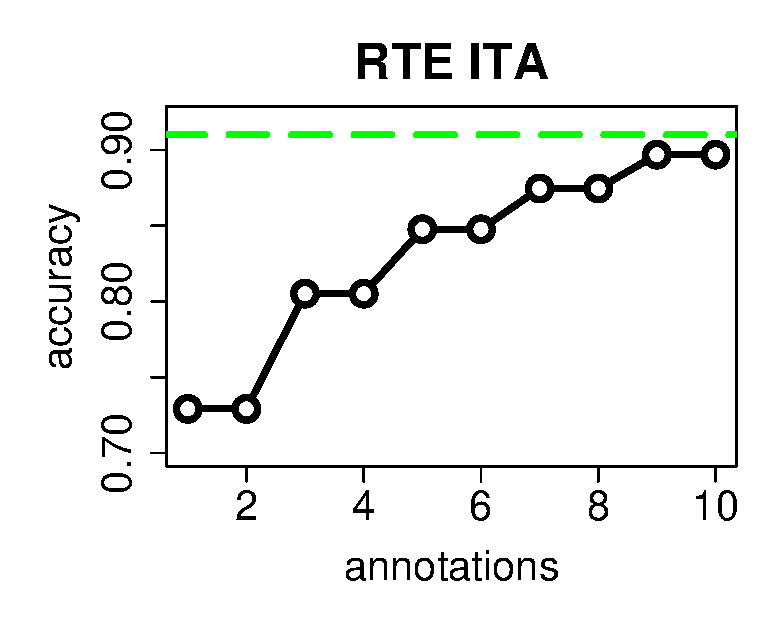
\includegraphics[width=7cm]{figures/rte.eps}
\caption{Inter-annotator agreement for RTE experiment } \label{rteITA}
\end{figure}
%RTE 3
%\cite{rte3}
%Also, we are able to do a further analysis of the results obtained in \cite{Zaenen:08}.

%\subsection{ Subjectivity Analysis? }
%Possible corpus: http://www.cs.pitt.edu/~wiebe/pubs/pub4.html
%MPQA Opinion Corpus annotated for opinions and sentiments

%\subsection{ Coreference Resolution? }
%Possible corpus:  MUC-6, MUC-7, ACE

\subsection{Event Annotation}

This task is inspired by the TimeBank corpus \cite{TimeBank}, which includes among its annotations
a label for event-pairs that represents the temporal relation between them, from a set of fourteen relations ({\em before}, {\em after}, {\em during}, {\em includes}, etc.).
%The TimeBank corpus consists of (X) sentences with Y labeled verb events;  these verb events have labeled with respect to neighboring verb events into one of six categories:  ()...
% [[ Explain the different even annotations:  before, after, overlapping, etc]]
We implement \textit{temporal ordering} as a simplified version of the TimeBank event temporal annotation task: rather than annotating all fourteen event types, we restrict our consideration to the two simplest labels:  ``strictly before'' and ``strictly after''.  Furthermore, rather than marking both nouns and verbs in the text as possible events, we only consider possible verb events.  We extract the 462 verb event pairs labeled as ``strictly before'' or ``strictly after'' in the TimeBank corpus, and we present these  pairs to annotators with a forced binary choice on whether the event described by the first verb occurs \textit{before} or \textit{after} the second.  For example, in a dialogue about a plane explosion, we have the utterance:  ``\textit{It just blew up in the air, and then we saw two fireballs go down to the, to the water, and there was a big small, ah, smoke, from ah, coming up from that}''.  Here for each annotation we highlight the specific verb pair of interest (e.g., \textit{go}/\textit{coming}, or \textit{blew}/\textit{saw}) and ask which event occurs first (here, \textit{go} and \textit{blew}, respectively).

The results of this task are presented in Figure \ref{tempITA}.  We achieve high agreement for this task, at a rate of 0.94 with simple voting over 10 annotators (4620 total annotations). While an expert ITA of 0.77 was reported for the more general task involving all fourteen labels on both noun and verb events, no expert ITA numbers have been reported for this simplified temporal ordering task.
%This was by far the most expensive of the five tasks, at total cost of \$13.82, a rate of only 333 annotations per USD .  
\begin{figure}[ht]
\centering
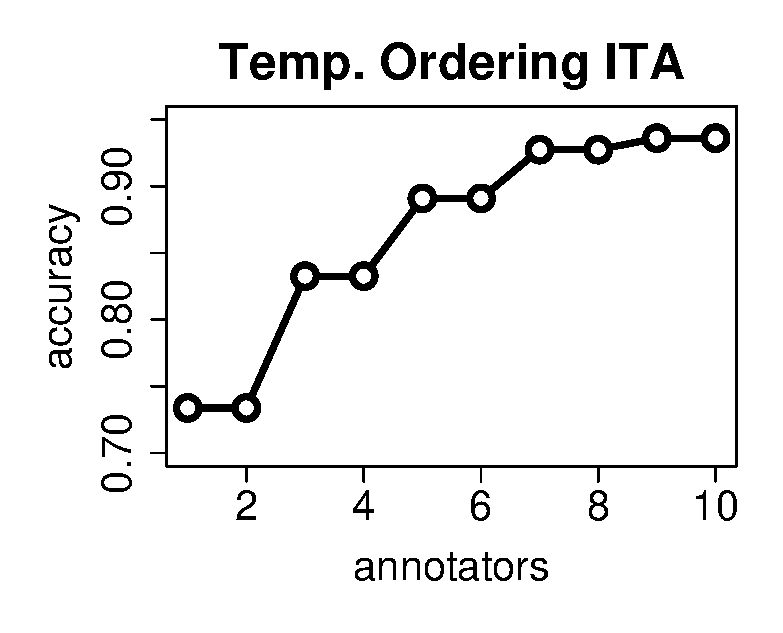
\includegraphics[width=7cm]{figures/temp.eps}
\caption{ITA for temporal ordering experiment } \label{tempITA}
\end{figure}
\vspace*{-0.2in}
%Second, we give annotators the set of all labeled Timebank relations, and we ask for \textit{before}, \textit{after}, and \textit{other} labels.  Here we emphasize the notion of \textit{strictly before} and \textit{strictly after}.
%[[ Task example ]]
\subsection{ Word Sense Disambiguation }
In this task we consider a simple problem on which machine learning algorithms have been shown to produce extremely good results; here we annotate part of the SemEval Word Sense Disambiguation Lexical Sample task \cite{task17}; specifically, we present the labeler with a paragraph of text containing the word ``president'' (e.g., a paragraph containing ``\textit{Robert E. Lyons III...was appointed president  and chief operating officer...}'') and ask the labeler which one of the following three sense labels is most appropriate:\\
\small{1) \textit{executive officer of a firm, corporation, or university} \\
2) \textit{head of a country (other than the U.S.) } \\
3) \textit{head of the U.S., President of the United States} } \\
\normalsize We collect 10 annotations for each of 177 examples of the noun ``president'' for the three senses given in SemEval.  As shown in Figure \ref{wsdITA}, performing simple majority voting (with random tie-breaking) over annotators results in a rapid accuracy plateau at a very high rate of 0.994 accuracy.  In fact, further analysis reveals that there was only a single disagreement between the averaged non-expert vote and the gold standard; on inspection it was observed that the annotators voted strongly against the original gold label (9-to-1 against), and that it was in fact found to be an error in the original gold standard annotation.\footnote{The example sentence began ``\textit{The Egyptian president said he would visit Libya today...}'' and was mistakenly marked as the ``head of a company'' sense in the gold annotation (example id 24:0@24@wsj/23/wsj\_2381@wsj@en@on).}  
After correcting this error, the non-expert accuracy rate is 100\% on the 177 examples in this task.  This is a specific example where non-expert annotations can be used to correct expert annotations.

Since expert ITA was not reported per word on this dataset, we compare instead to the performance of the best automatic system performance for disambiguating ``president'' in SemEval Task 17 \cite{Cai:07}, with an accuracy of 0.98.  %1770 annotations was collected as a price of US\$1.76, a rate of 1005.7 annotations per USD.

\begin{figure}[ht]
\centering
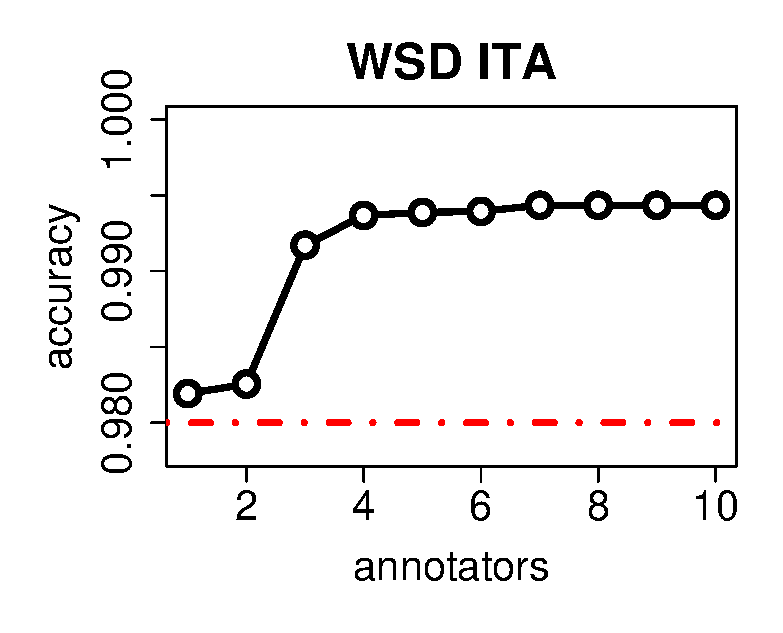
\includegraphics[width=7cm]{figures/wsd.eps}
\caption{Inter-annotator agreement for WSD experiment } \label{wsdITA}
\end{figure}


%\subsection{ Machine Translation Evaluation?
%Possible corpus:  GALE HTER evaluations
%  better:  fluency / adequacy judgments.  another day...

\subsection{ Summary }

\begin{table}[h]
\footnotesize
    \begin{center}
        \begin{tabular}{|c||c|c|c|c|c|}
        \hline
        & & Cost & Time & Labels & Labels \\
        Task & Labels  & (USD) & (hrs) & per USD & per hr \\
        \hline
        Affect & 7000 & \$2.00 & 5.93 & 3500 & 1180.4 \\
        WSim & 300 & \$0.20 & 0.174 & 1500 & 1724.1 \\
        RTE & 8000 & \$8.00 & 89.3 & 1000 & 89.59 \\
       % RTE3 &  &  & -- & -- \\
        Event & 4620 & \$13.86 & 39.9 & 333.3 & 115.85 \\
        WSD & 1770 & \$1.76 & 8.59 & 1005.7 & 206.1  \\
        \hline
        Total & 21690 & 25.82 & 143.9 & 840.0 & 150.7 \\
        \hline
        \end{tabular}
    \caption{Summary of costs for non-expert labels}\label{costs}
\end{center}
\end{table}

In Table \ref{costs} we give a summary of the costs associated with
obtaining the non-expert annotations for each of our 5 tasks.  Here
\textit{Time} is given as the total amount of time in hours elapsed
from submitting the group of HITs to AMT until the last assignment
is submitted by the last worker.  %We observe that in general we
%collect fewer answers for categorical tasks (RTE, Event, WSD) 
%than for numeric response tasks despite the fact that we offered more money per label.
%We expect that this is due to the increased cognitive load of those tasks.

\section{ Bias correction for non-expert annotators  }

The reliability of individual workers varies.  Some are very accurate, while others are more careless and make mistakes; and a small few give very noisy responses.  Furthermore, for most AMT data collection experiments, a relatively small number of workers do a large portion of the task, since workers may do as much or as little as they please.  Figure \ref{Workers} shows accuracy rates for individual workers on one task.  Both the overall variability, as well as the prospect of identifying high-volume but low-quality workers, suggest that controlling for individual worker quality could yield higher quality overall judgments.

\begin{figure}[t]
\centering
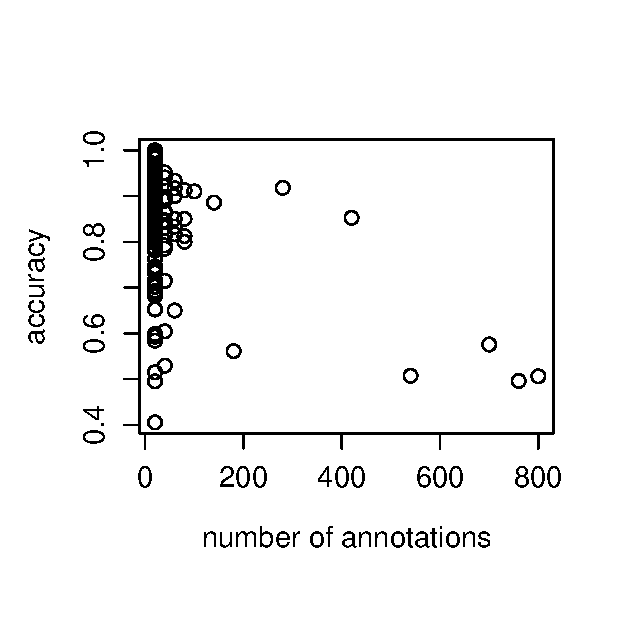
\includegraphics[width=6cm]{figures/workers.eps}
\caption{Worker accuracies on the RTE task.  Each point is one worker.  Vertical jitter has been added to points on the left to show the large number of workers who did the minimum amount of work (20 examples).} \label{Workers}
\end{figure}
In general, there are at least three ways to enhance quality in the face of worker error.  More workers can be used, as described in previous sections.  
%\footnote{\newcite{Sheng:08} experiment with various strategies to approach data collection of noisy labels.}
Another method is to use Amazon's compensation mechanisms to give monetary bonuses to highly-performing workers and deny payments to unreliable ones; this is useful, but beyond the scope of this paper.  In this section we explore a third alternative, to model the reliability and biases of individual workers and correct for them.

A wide number of methods have been explored to correct for the bias of annotators.  \newcite{Dawid:79} are the first to consider the case of having multiple annotators per example but unknown true labels.  They introduce an EM algorithm to simultaneously estimate annotator biases and latent label classes.  \newcite{Wiebe:99} analyze linguistic annotator agreement statistics to find bias, and use a similar model to correct labels.  A large literature in biostatistics addresses this same problem for medical diagnosis.  \newcite{Albert:04} review several related models, but argue they have various shortcomings and emphasize instead the importance of having a gold standard.

%\footnote{At the time of this writing, Bob Carpenter is experimenting with our data in Gibbs sampling versions of these models (e.g. Carpenter, 2008); see \texttt{\scriptsize{http://lingpipe-blog.com}} and \texttt{\scriptsize{http://blog.doloreslabs.com/topics/wisdom/}} for updates.}

Here we take an approach based on gold standard labels, using a small amount of expert-labeled training data in order to correct for the individual biases of different non-expert annotators.  The idea is to recalibrate worker's responses to more closely match expert behavior.  We focus on categorical examples, though a similar method can be used with numeric data.
\vspace*{-0.1in}
\subsection{ Bias correction in categorical data }

Following Dawid and Skene, we model labels and workers with a multinomial model similar to Naive Bayes.
Every example $i$ has a true label $x_i$.  For simplicity, assume two labels $\{Y,N\}$.   Several different workers give labels $y_{i1}, y_{i2}, \ldots y_{iW}$.  A worker's conditional probability of response is modeled as multinomial, and we model each worker's judgment as conditionally independent of other workers given the true label $x_i$, i.e.:
\[ P(y_{i1}, \ldots, y_{iW}, x_i) = \left( \prod_{w} P(y_{iw} | x_i) \right) p(x_i) \]

To infer the posterior probability of the true label for a new example, worker judgments are integrated via Bayes rule, yielding the posterior log-odds:
\begin{eqnarray*}
&& \log \frac{P(x_i = Y  | y_{i1} \ldots y_{iW}) }{ P(x_i=N | y_{i1} \ldots y_{iW})  }  \\
&=& \sum_w \log \frac{ P(y_{iw} | x_i = Y) }{ P(y_{iw} | x_i = N) } + \log \frac{P(x_i=Y)}{P(x_i=N)} \\
\end{eqnarray*}

The worker response likelihoods $P(y_w | x=Y)$ and $P(y_w | x=N)$ can be directly estimated from frequencies of worker performance on gold standard examples.  
(If we used maximum likelihood estimation with no Laplace smoothing, then each $y_w | x$ is just the worker's empirical confusion matrix.)  For MAP label estimation, the above equation describes a weighted voting rule: each worker's vote is weighted by their log likelihood ratio for their given response.  Intuitively, workers who are more than 50\% accurate have positive votes; workers whose judgments are pure noise have zero votes; and anticorrelated workers have negative votes.  (A simpler form of the model only considers accuracy rates, thus weighting worker votes by $\log \frac{\textrm{acc}_w}{1-\textrm{acc}_w}$.  But we use the full unconstrained multinomial model here.)

\subsubsection{ Example tasks: RTE-1 and event annotation }

We used this model to improve accuracy on the RTE-1 and event annotation tasks.  (The other categorical task, word sense disambiguation, could not be improved because it already had maximum accuracy.)  First we took a sample of annotations giving $k$ responses per example.  Within this sample, we trained and tested via 20-fold cross-validation across examples.  Worker models were fit using Laplace smoothing of 1 pseudocount; label priors were uniform, which was reasonably similar to the empirical distribution for both tasks.

\begin{figure}[ht]
\centering
\includegraphics[width=8cm]{figures/goldcalib.eps}
\caption{Gold-calibrated labels versus raw labels} \label{WorkerModelResults}
\end{figure}

Figure \ref{WorkerModelResults} shows improved accuracy at different numbers of annotators.  The lowest line is for the naive 50\% majority voting rule.  (This is equivalent to the model under uniform priors and equal accuracies across workers and labels.)  Each point is the data set's accuracy against the gold labels, averaged across resamplings each of which obtains $k$ annotations per example.  RTE has an average +4.0\% accuracy increase, averaged across 2 through 10 annotators.  We find a +3.4\% gain on event annotation.
Finally, we experimented with a similar calibration method for numeric data, using a Gaussian noise model for each worker: $y_w | x \sim N(x + \mu_w, \sigma_w)$.  On the affect task, this yielded a small but consistent increases in Pearson correlation at all numbers of annotators, averaging a +0.6\% gain.

\section{ Training a system with non-expert annotations }

In this section we train a supervised affect recognition system with expert vs. non-expert annotations.

\subsection{ Experimental Design }

For the purpose of this experiment we create a simple bag-of-words unigram model for predicting affect and valence, similar to the SWAT system \cite{SWAT}, one of the top-performing systems on the SemEval Affective Text task.\footnote{ Unlike the SWAT system we perform no lemmatization, synonym expansion, or any other preprocessing of the tokens;  we simply use whitespace-separated tokens within each headline.} For each token $t$ in our training set, we assign $t$ a weight for each emotion $e$ equal to the average emotion score observed in each headline $H$ that $t$ participates in. i.e., if $\mathbf{H}_t$ is the set of headlines containing the token $t$, then:

\begin{equation*}
Score(e,t) = \frac{ \sum_{ H \in \mathbf{H}_t } Score(e,H) }{ | \mathbf{H}_t | }
\end{equation*}

With these weights of the individual tokens we may then compute the score for an emotion $e$ of a new headline $H$ as the average score over the set of tokens $t \in H$ that we've observed in the training set (ignoring those tokens not in the training set), i.e.:

\begin{equation*}
Score(e,H) = \sum_{ t \in H} \frac{ Score(e,t) }{ | H |}
\end{equation*}

Where $|H|$ is simply the number of tokens in headline $H$, ignoring tokens not observed in the training set.

\subsection{ Experiments }

%First we verify that our model gives reasonable performance on the full task, trained and evaluated on the gold standard labels:
We use 100 headlines as a training set (examples 500-599 from the test set of SemEval Task 14),  and we use the remaining 900 headlines as our test set. Since we are fortunate to have the six separate expert annotations in this task, we can perform an extended systematic comparison of the performance of the classifier trained with expert vs. non-expert data.

\begin{table}[h]
\footnotesize
    \begin{center}
        \begin{tabular}{|c||c|c|c|c|}
        \hline
        %BTO more explicit
        Emotion & 1-Expert & 10-NE & $k$ & $k$-NE \\
        \hline
        Anger & 0.084 & 0.233 & 1 & 0.172 \\
        Disgust & 0.130 & 0.231 & 1 & 0.185 \\
        Fear & 0.159 & 0.247 & 1 & 0.176 \\
        Joy & 0.130 & 0.125 & -- & -- \\
        Sadness & 0.127 & 0.174 & 1 & 0.141 \\
        Surprise & 0.060 & 0.101 & 1 & 0.061 \\
        Valence & 0.159 & 0.229 & 2 & 0.146 \\
        \hline
        Avg. Emo & 0.116 & 0.185 & 1 & 0.135 \\
        Avg. All & 0.122 & 0.191 & 1 & 0.137 \\
        \hline
        \end{tabular}

    \caption{Performance of expert-trained and non-expert-trained classifiers on test-set.  $k$ is the minimum number of non-experts needed to beat an average expert.}\label{affectSWAT}
\end{center}
\end{table}
%\vspace*{\tableReduceBot}

For this evaluation we compare the performance of systems
trained on expert and non-expert annotations.
For each expert annotator we train a system using only
the judgments provided by that annotator, and then create a gold
standard test set using the average of the responses of the remaining
five labelers on that set.  In this way we create six independent
expert-trained systems and compute the average across their
performance, calculated as Pearson correlation to the gold standard;
this is reported in the ``1-Expert'' column of Table \ref{affectSWAT}.

Next we train systems using non-expert labels;  for each possible
subset of $n$ annotators, for $n \in \{1, 2, \ldots, 10\}$ we
train a system, and evaluate by calculating Pearson correlation
with the same set of gold standard datasets used in the expert-trained
system evaluation. Averaging the results of these studies yields the results in Table \ref{affectSWAT}. %and in figure [[figure]].

As in Table \ref{affectITA2} we calculate the minimum number of
non-expert annotations per example $k$ required on average to achieve
similar performance to the expert annotations; surprisingly we find
that for five of the seven tasks, the average system trained with
a single set of non-expert annotations outperforms the average
system trained with the labels from a single expert.  One possible
hypothesis for the cause of this non-intuitive result is that
individual labelers (including experts) tend to have a strong bias,
and since multiple non-expert labelers may contribute to a single
set of non-expert annotations, the annotator diversity within the
single set of labels may have the effect of reducing annotator bias
and thus increasing system performance.
\vspace*{-0.1in}
\section{Conclusion}

We demonstrate the effectiveness of using Amazon Mechanical Turk
for a variety of natural language annotation tasks.  Our evaluation of non-expert labeler data vs. expert annotations for five tasks found that for many tasks only a small number of non-expert
annotations per item are necessary to equal the performance of an expert annotator.  
In a detailed study of expert and non-expert agreement for an affect recognition task we find
that we require an average of 4 non-expert labels per item in order
to emulate expert-level label quality. Finally, we demonstrate significant improvement by controlling for labeler bias.

\subsection*{Acknowledgments}
Thanks to Nathanael Chambers, Annie Zaenen, Rada Mihalcea, Qi Su, Panos Ipeirotis, Bob Carpenter, David Vickrey, William Morgan, and Lukas Biewald for useful discussions, and for the generous support of Dolores Labs.  This work was supported in part by the Disruptive Technology Office (DTO)'s Advanced Question Answering for Intelligence (AQUAINT) Phase III Program.

\bibliographystyle{acl}
\begin{thebibliography}{}%\denselist

%@inproceedings{1034721,
% author = {Janyce M. Wiebe and Rebecca F. Bruce and Thomas P. O'Hara},
% title = {Development and use of a gold-standard data set for subjectivity classifications},
% booktitle = {Proceedings of the 37th annual meeting of the Association for Computational Linguistics on Computational Linguistics},
% year = {1999},
% isbn = {1-55860-609-3},
% pages = {246--253},
% location = {College Park, Maryland},
% doi = {http://dx.doi.org/10.3115/1034678.1034721},
% publisher = {Association for Computational Linguistics},
% address = {Morristown, NJ, USA},
% }

\bibitem[\protect\citename{Albert and Dodd}2004]{Albert:04}
Paul S. Albert and Lori E. Dodd.
\newblock 2004.
\newblock A Cautionary Note on the Robustness of Latent Class Models for Estimating Diagnostic Error without a Gold Standard. 
%\newblock In \textit{Proc. of COLING-ACL 1998}.
\newblock Biometrics, Vol. 60 (2004), pp. 427-435.
%Applied Statistics, Vol. 28, No. 1 (1979), pp. 20-28.


\bibitem[\protect\citename{Baker et al.}1998]{FrameNet}
Collin F. Baker, Charles J. Fillmore and John B. Lowe.
\newblock 1998.
\newblock The Berkeley FrameNet project. 
\newblock In \textit{Proc. of COLING-ACL 1998}.

\bibitem[\protect\citename{Banko and Brill}2001]{Banko:01}
Michele Banko and Eric Brill.
\newblock 2001.
\newblock Scaling to Very Very Large Corpora for Natural Language Disambiguation.
\newblock In \textit{Proc. of ACL-2001}.

\bibitem[\protect\citename{Cai et al.}2007]{Cai:07}
Junfu Cai, Wee Sun Lee and Yee Whye Teh.
\newblock 2007.
\newblock Improving Word Sense Disambiguation Using Topic Features.
\newblock In \textit{ Proc. of EMNLP-2007 }.

%\bibitem[\protect\citename{Carpenter}2008]{CarpenterPoster}
%Bob Carpenter.
%\newblock 2008.
%\newblock Hierarchical Bayesian Models of Categorical Data Analysis. 
%\newblock Poster in \textit{ New York Academy of Sciences 3rd Annual Machine Learning Symposium}.
%\newblock Writeup online: \texttt{\scriptsize{http://lingpipe-blog.com/2008/09/05/hierarchical-bayesian-models-of-categorical-data-annotation/}}

\bibitem[\protect\citename{Chklovski and Mihalcea}2002]{WordExpert}
Timothy Chklovski and Rada Mihalcea.
\newblock 2002.
\newblock Building a sense tagged corpus with Open Mind Word Expert. 
\newblock In \textit{ Proc. of the Workshop on "Word Sense Disambiguation: Recent Successes and Future Directions", ACL 2002}.

\bibitem[\protect\citename{Chklovski and Gil}2005]{Chklovski:05}
Timothy Chklovski and Yolanda Gil.
\newblock 2005.
\newblock Towards Managing Knowledge Collection from Volunteer Contributors.
\newblock Proceedings of AAAI Spring Symposium on Knowledge Collection from Volunteer Contributors (KCVC05).

%\bibitem[\protect\citename{Chklovski and Mihalcea}2003]{Chklovski:03}
%Timothy Chklovski and Rada Mihalcea.
%\newblock 2003.
%\newblock Exploiting Agreement and Disagreement of Human Annotators for Word Sense Disambiguation.
%\newblock In {\it Proceedings of RANLP 2003}.

\bibitem[\protect\citename{Dagan et al.}2006]{rte1}
Ido Dagan, Oren Glickman and Bernardo Magnini. 
\newblock 2006.
\newblock The PASCAL Recognising Textual Entailment Challenge. 
\newblock Machine Learning Challenges. Lecture Notes in Computer Science, Vol. 3944, pp. 177-190, Springer, 2006.

\bibitem[\protect\citename{Dakka and Ipeirotis}2008]{Dakka:08}
Wisam Dakka and Panagiotis G. Ipeirotis.
\newblock 2008.
\newblock Automatic Extraction of Useful Facet Terms from Text Documents.
\newblock In \textit{Proc. of ICDE-2008}.

\bibitem[\protect\citename{Dawid and Skene}1979]{Dawid:79}
A. P. Dawid and A. M. Skene.
\newblock 1979.
\newblock Maximum Likelihood Estimation of Observer Error-Rates Using the EM Algorithm.
\newblock Applied Statistics, Vol. 28, No. 1 (1979), pp. 20-28.

%
%Christiane Fellbaum.
%\newblock 1998.
%\newblock WordNet: An Electronic Lexical Database.
%\newblock Cambridge, MA: MIT Press.

%\bibitem[\protect\citename{Giampiccolo et al.}2007]{rte3}
%Danilo Giampiccolo, Bernardo Magnini, Ido Dagan, and Bill Dolan.
%\newblock 2007.
%\newblock The third PASCAL recognizing textual entailment challenge.
%\newblock In \textit{ Proc. of Workshop on Textual Entailment and Paraphrasing, ACL-2007}.

%\bibitem[\protect\citename{Liu and Singh}2003]{ConceptNet}
%Hugo Liu and Push Singh.
%\newblock 2003.
%\newblock ConceptNet: A practical commonsense reasoning toolkit.
%\newblock BT Technology Journal, 22(4):211-226.

\bibitem[\protect\citename{Kaisser and Lowe}2008]{Kaisser:08a}
Michael Kaisser and John B. Lowe. 
\newblock 2008.
\newblock A Research Collection of Question–Answer Sentence Pairs.
\newblock In \textit{Proc. of LREC-2008}.

\bibitem[\protect\citename{Kaisser et al.}2008]{Kaisser:08b}
Michael Kaisser, Marti Hearst, and John B. Lowe. 
\newblock 2008.
\newblock Evidence for Varying Search Results Summary Lengths. 
\newblock In \textit{Proc. of ACL-2008}.

\bibitem[\protect\citename{Katz et al.}2007]{SWAT}
Phil Katz, Matthew Singleton, Richard Wicentowski. 
\newblock 2007.
\newblock SWAT-MP: The SemEval-2007 Systems for Task 5 and Task 14.
\newblock In \textit{ Proc. of SemEval-2007}.

\bibitem[\protect\citename{Kittur et al.}2008]{Kittur:08}
Aniket Kittur, Ed H. Chi, and Bongwon Suh. 
\newblock 2008.
\newblock Crowdsourcing user studies with Mechanical Turk. 
\newblock In \textit{ Proc. of CHI-2008}.

\bibitem[\protect\citename{Marcus et al.} 1993]{TreeBank}
Mitchell P. Marcus, Mary Ann Marcinkiewicz, and Beatrice Santorini.
\newblock 1993.
\newblock Building a large annotated corpus of English: the Penn Treebank.
\newblock Computational Linguistics 19:2, June 1993.

\bibitem[\protect\citename{Miller and Charles} 1991]{MC}
George A. Miller and William G. Charles.
\newblock 1991.
\newblock Contextual Correlates of Semantic Similarity.
\newblock Language and Cognitive Processes, vol. 6, no. 1, pp. 1-28, 1991.

\bibitem[\protect\citename{Miller et al.} 1993]{SemCor}
George A. Miller, Claudia Leacock, Randee Tengi, and Ross T. Bunke.
\newblock 1993.
\newblock A semantic concordance.
\newblock In \textit{Proc. of HLT-1993}.

\bibitem[\protect\citename{Nakov}2008]{NakovLREC:08}
Preslav Nakov.
\newblock 2008.
\newblock Paraphrasing Verbs for Noun Compound Interpretation.
\newblock In \textit{Proc. of the Workshop on Multiword Expressions, LREC-2008}.

%\bibitem[\protect\citename{Nakov and Hearst}2008]{NakovACL:08}
%Preslav Nakov and Marti A. Hearst.
%\newblock 2008.
%\newblock Solving Relational Similarity Problems Using the Web as a Corpus.
%\newblock In \textit{Proc. of ACL-2008}.

\bibitem[\protect\citename{Palmer et al.}2005]{PropBank}
Martha Palmer, Dan Gildea, and Paul Kingsbury.
\newblock 2005.
\newblock The Proposition Bank: A Corpus Annotated with Semantic Roles.
\newblock Computational Linguistics, 31:1.

\bibitem[\protect\citename{Pradhan et al.} 2007]{task17}
Sameer Pradhan, Edward Loper, Dmitriy Dligach and Martha Palmer. 
\newblock 2007.
\newblock SemEval-2007 Task-17: English Lexical Sample, SRL and All Words. 
\newblock In \textit{ Proc. of SemEval-2007 }.

\bibitem[\protect\citename{Pustejovsky et al.}2003]{TimeBank}
James Pustejovsky, Patrick Hanks, Roser Saurí, Andrew See, Robert Gaizauskas, Andrea Setzer, Dragomir Radev, Beth Sundheim, David Day, Lisa Ferro and Marcia Lazo.
\newblock 2003.
\newblock The TIMEBANK Corpus. 
\newblock In \textit{Proc. of Corpus Linguistics 2003, 647-656.}

\bibitem[\protect\citename{Resnik}1999]{Resnik:99}
Philip Resnik. 
\newblock 1999.
\newblock Semantic Similarity in a Taxonomy: An Information-Based Measure and its Application to Problems of Ambiguity in Natural Language.
\newblock JAIR, Volume 11, pages 95-130.

\bibitem[\protect\citename{Rubenstein and Goodenough}1965]{RG}
Herbert Rubenstein and John B. Goodenough.
\newblock 1965.
\newblock Contextual Correlates of Synonymy.
\newblock Communications of the ACM, 8(10):627--633.

\bibitem[\protect\citename{Sheng et al.}2008]{Sheng:08}
Victor S. Sheng, Foster Provost, and Panagiotis G. Ipeirotis.
\newblock 2008.
\newblock Get Another Label? Improving Data Quality and Data Mining Using Multiple, Noisy Labelers.
\newblock In \textit{Proc. of KDD-2008.}

\bibitem[\protect\citename{Singh}2002]{OpenMindCommonSense}
Push Singh.
\newblock 2002. 
\newblock The public acquisition of commonsense knowledge.
\newblock In \textit{Proc. of AAAI Spring Symposium on Acquiring (and Using) Linguistic (and World) Knowledge for Information Access, 2002.}

\bibitem[\protect\citename{Sorokin and Forsyth}2008]{Sorokin:08}
Alexander Sorokin and David Forsyth.
\newblock 2008.
\newblock Utility data annotation with Amazon Mechanical Turk.
\newblock To appear in \textit{Proc. of First IEEE Workshop on Internet Vision at CVPR, 2008.}
\newblock See also: \texttt{\scriptsize{http://vision.cs.uiuc.edu/annotation/}}

\bibitem[\protect\citename{Stork}1999]{OpenMind}
David G. Stork.
\newblock 1999. 
\newblock The Open Mind Initiative.
\newblock IEEE Expert Systems and Their Applications pp. 16-20, May/June 1999.

\bibitem[\protect\citename{Strapparava and Mihalcea}2007]{AffectiveText}
Carlo Strapparava and Rada Mihalcea.
\newblock 2007.
\newblock SemEval-2007 Task 14: Affective Text
\newblock In \textit{Proc. of SemEval-2007}.

\bibitem[\protect\citename{Su et al.}2007]{Su:07}
Qi Su, Dmitry Pavlov, Jyh-Herng Chow, and Wendell C. Baker.
\newblock 2007.
\newblock Internet-Scale Collection of Human-Reviewed Data. 
\newblock In \textit{Proc. of WWW-2007}.

\bibitem[\protect\citename{von Ahn and Dabbish}2004]{espgame}
Luis von Ahn and Laura Dabbish.
\newblock 2004.
\newblock Labeling Images with a Computer Game.
\newblock In ACM Conference on Human Factors in Computing Systems, CHI 2004.

\bibitem[\protect\citename{von Ahn et al.}2006]{verbosity}
Luis von Ahn, Mihir Kedia and Manuel Blum. 
\newblock 2006.
\newblock Verbosity: A Game for Collecting Common-Sense Knowledge. 
\newblock In ACM Conference on Human Factors in Computing Systems, CHI Notes 2006.

\bibitem[\protect\citename{Voorhees and Dang}2006]{Voorhees:06}
Ellen Voorhees and Hoa Trang Dang.
\newblock 2006.
\newblock Overview of the TREC 2005 question answering track.
\newblock In \textit{ Proc. of TREC-2005}.

\bibitem[\protect\citename{Wiebe et al.}1999]{Wiebe:99}
Janyce M. Wiebe, Rebecca F. Bruce and Thomas P. O'Hara.
\newblock 1999.
\newblock Development and use of a gold-standard data set for subjectivity classifications.
\newblock In \textit{Proc. of ACL-1999}.

\bibitem[\protect\citename{Zaenen}Submitted]{Zaenen:08}
Annie Zaenen. 
\newblock Submitted.  % bto: "2008" ?
\newblock Do give a penny for their thoughts.
\newblock International Journal of Natural Language Engineering (submitted).

\end{thebibliography}

\end{document}
